\documentclass[14pt, t]{beamer}
\usetheme{default}
\beamertemplatenavigationsymbolsempty
\setbeamertemplate{note page}[plain]
\setbeamertemplate{frametitle}
{
\begin{flushleft}
\textbf{\insertframetitle}
\end{flushleft}
}

% \documentclass[12pt]{article}
% \usepackage[margin=1in]{geometry}
% \usepackage{graphicx}
% \usepackage{titling}
% \renewenvironment{frame}[1]{\noindent\textbf{#1}}{\medskip}
% \renewcommand{\titlepage}{\large\textbf{\thetitle} --- \thedate\bigskip}

\usepackage{amsmath}
\usepackage{amssymb}

\DeclareMathOperator{\G}{G}
\DeclareMathOperator{\N}{N}
% \DeclareMathOperator{\Pr}{\Pr}
\DeclareMathOperator{\Uniform}{Uniform}

\title{\textbf{Bayesian Methods in Election Forecasting}}
\author{Michael Maltese, advisor Gabriel Chandler}
\date{31 January 2014}

\begin{document}

\begin{frame}
\titlepage
\end{frame}

\begin{frame}{How does it work?}
\begin{itemize}
	\item Basic information ahead of time (what's the economy like? how many people are dying?)
	\item Incorporate opinion polls
	\item Estimate state outcomes (the electoral college)
\end{itemize}
\end{frame}

\begin{frame}{Motivation}
\begin{itemize}
	\item Statistics can do a better job at political punditry
	\item Suppose you're a political campaign. How do you spend your money?
\end{itemize}
\end{frame}

\begin{frame}{Motivation}
\begin{itemize}
	\item Consider swing states. It's probably better to assign resources to states that are close, than to states that are not (taking the electoral college into account).
	\item Figure out what states are/will be swing states
\end{itemize}
\end{frame}

\begin{frame}{Before opinion polls}
\begin{itemize}
	\item We can predict presidential elections ahead of time using various indicators.
	\item My favorite: \textbf{Bread-and-Peace}. How is the economy doing, and how many military personnel have died recently?
\end{itemize}
\end{frame}

\begin{frame}{Before opinion polls}
\begin{itemize}
\item Linear regression: given a model of the form
\begin{equation*}
		vote = \beta_0 + \beta_1\cdot bread + \beta_2\cdot peace + \epsilon,
	\end{equation*}
	we can estimate \(\beta\)s using historical data and predict upcoming elections.
\end{itemize}
\end{frame}

\begin{frame}[c]
\begin{center}
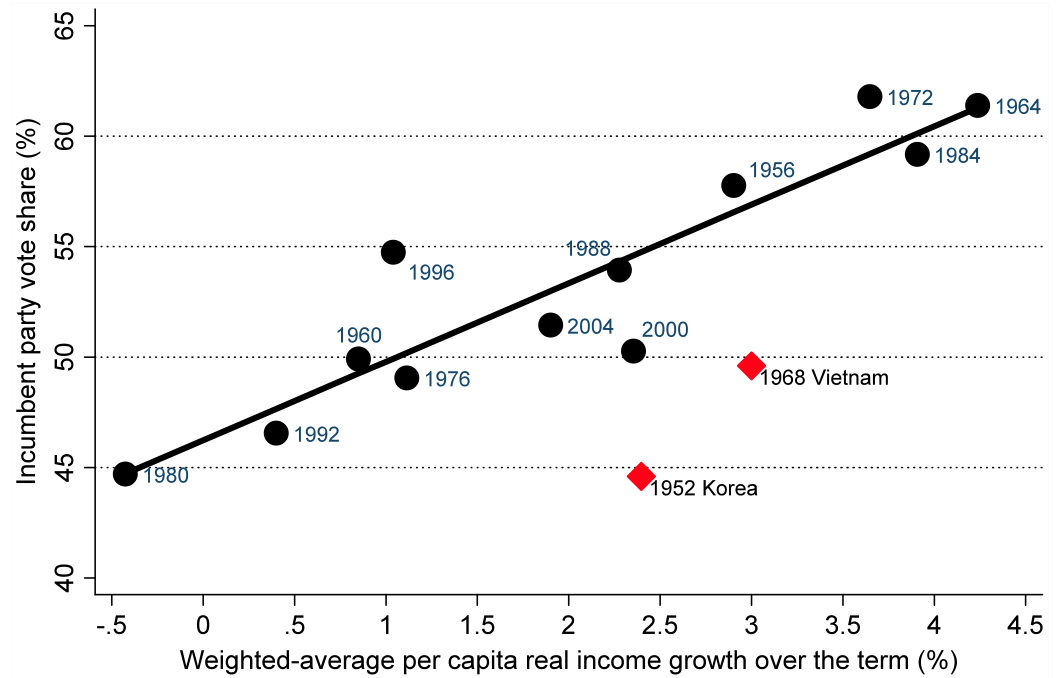
\includegraphics[width=\textwidth]{bread-and-peace.png}
\end{center}
\end{frame}

\begin{frame}{National vs. state elections}
\begin{itemize}
	\item Popular vote means nothing! Presidents must win the Electoral College. (Assume if you win the popular vote in a state, you get all of its Electoral College votes. Not always true.)
	\item Need to actually forecast \emph{state} results
\end{itemize}
\end{frame}

\begin{frame}{States before opinion polls}
\begin{itemize}
	\item You could use a linear regression, as before.
\end{itemize}
\end{frame}

\begin{frame}{States before opinion polls}
\begin{itemize}
	\item You could use a linear regression, as before.
	\item Or, states' deviations from the national vote are relatively stable between elections:
\end{itemize}
	\begin{center}
	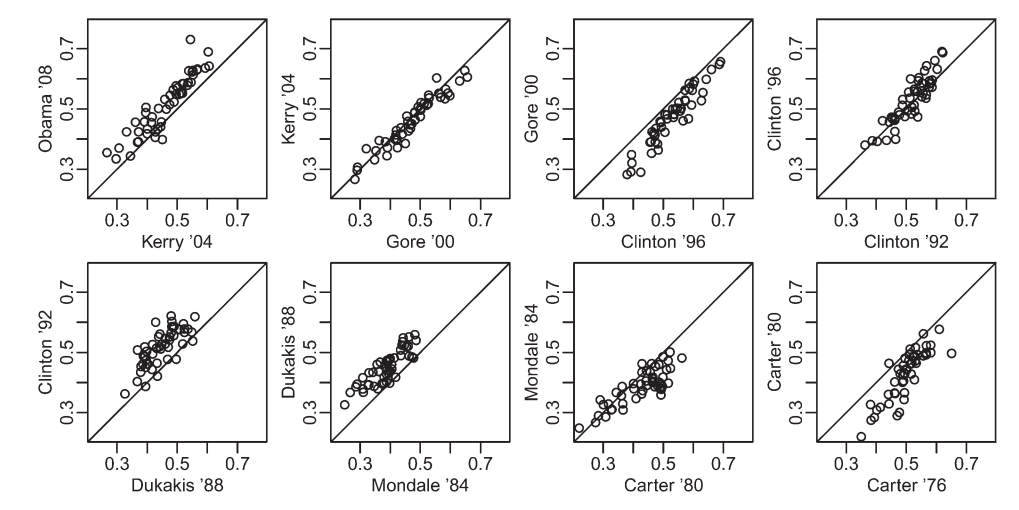
\includegraphics[width=\textwidth]{statestability.png}
	\end{center}
\end{frame}

\begin{frame}{Multi-level regression}
\begin{itemize}
	\item Also called mixed-effects. (If you know what fixed-effects is, it's a way of balancing that and no effects).
	\item Takes advantage of both within-group and between-group information
	\item If a group has very little data (like, state deviations from national vote over the last seven elections), it's ``shrunk'' towards the overall mean.
\end{itemize}
\end{frame}

\begin{frame}{Multi-level regression}
\begin{itemize}
	\item Looks like: \begin{align*}
		&deviation_i = \beta_0 + \epsilon_{state} + \epsilon_i
	\end{align*}
	\item ...which gives distributions on how much we believe each state may deviate.
	\item Technique also used in education, demographics, and geographical data
\end{itemize}
\end{frame}

\begin{frame}{Multi-level regression}
\begin{center}
	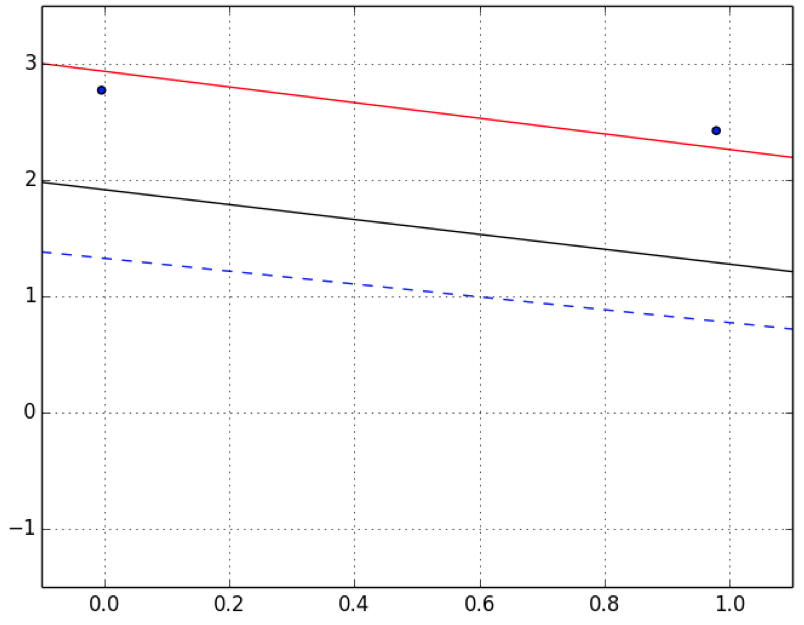
\includegraphics[width=0.8\textwidth]{mixed-effects.png}
	\end{center}
\end{frame}

\begin{frame}{Incorporating opinion polls}
\begin{itemize}
\item National and state-level
\item Different organizations (Gallup, Rasmussen, PPP, etc.)
\item Who do you sample? Will they change their minds between now and November?
\item Organizational biases and inaccuracies: e.g. maybe you think white male voters are going to be a larger proportion of the electorate than they turn out to be.
\end{itemize}
\end{frame}

\begin{frame}{Incorporating more data: Bayesian inference}
\begin{itemize}
	\item We call our predictions from before our \emph{prior distributions}
	\item Bayes' rule lets us update these probability distributions based on new information
\end{itemize}
\begin{align*}
		&\Pr(\theta|x) = \frac{\Pr(x|\theta) \Pr(\theta)}{\Pr(x)} \\
		&posterior \propto data \cdot prior
	\end{align*}
\end{frame}

\begin{frame}{Bayesian inference example}
Suppose you think a coin is pretty fairly weighted. You flip it four times, and get heads, heads, tails, heads.
\begin{center}
\includegraphics[height=0.5\textheight]{bayes-example.pdf}
\end{center}
\end{frame}

\begin{frame}{Incorporating opinion polls}
Suppose a poll \(y\) is centered on the result of the election, \(\alpha\), with some amount of variance \(\sigma^2\), and we also have a prior belief on the result of the election, \(\alpha\), which is centered at \(\mu\) with some variance \(\nu^2\). Bayes' rule tells us that
\begin{center}
 \[
		\alpha | y_i \sim \N\left[\left(\frac{\mu}{\nu^2} + \frac{y}{\sigma^2}\right)\left(\frac{1}{\nu^2} + \frac{1}{\sigma^2}\right)^{-1}, \left(\frac{1}{\nu^2} + \frac{1}{\sigma^2}\right)^{-1} \right]
	\]
\end{center}
\end{frame}

\begin{frame}{Incorporating opinion polls}
\begin{itemize}
	\item How do we find out that variance term? Or, how much information does a a poll has? (the variance from the election result)
	\item House biases
	\item Low reliability earlier in a campaign year
\end{itemize}
\end{frame}

\begin{frame}{Problem: House Biases}
\begin{itemize}
	\item Assume they cancel each other out (sum to 0)
	\item Ignore them?
	\item Use information from previous elections
	\item Figure it out during a campaign (more on this later)
\end{itemize}
\end{frame}

\begin{frame}{Problem: How reliable are polls in February?}
\begin{itemize}
	\item Not very.
	\item Empirical methods of figuring out reliability: regression, maximum likelihood estimation.
	\item Theoretical methods: modeling opinion as random walk
\end{itemize}
\end{frame}

\begin{frame}
\begin{center}
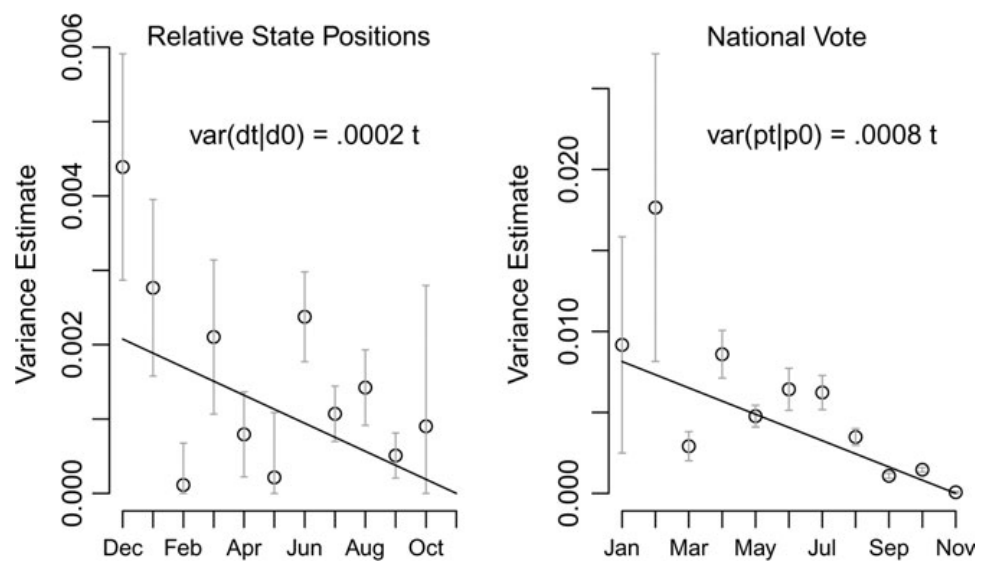
\includegraphics[width=\textwidth]{bayescombo_timevariance.png}
\end{center}
\end{frame}

\begin{frame}{Random walks}
\begin{itemize}
	\item Suppose that, each time period, who would be elected if the vote happened right now changes a little bit. \[\alpha_{t+1} \sim \N(\alpha_t, \omega^2)\]
	And polls are now centered around opinion at that time: \[
		y_i \sim N(\alpha_t, \sigma_i^2)
	\]
\end{itemize}
% Preference: if the election were held today, \alpha is what the vote would be.
% Hope the real data looks like this
\end{frame}

\begin{frame}{Random walks}	
\begin{center}
	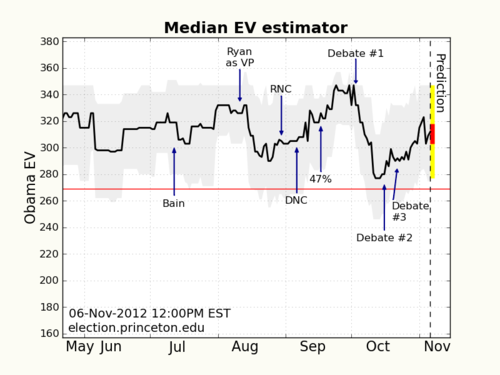
\includegraphics[width=0.8\textwidth]{EV_history.png}
\end{center}
\end{frame}

\begin{frame}{Random walks}
	\begin{itemize}
		\item Seems like a reasonable model.
		\item Now we have way too many variables!
		\item Solution: Gibbs sampling
	\end{itemize}
\end{frame}

\begin{frame}{Gibbs sampling}
\begin{itemize}
	\item When you have many variables which depend on each other
	\item For each variable in turn, assume that you know what every other variable is (use the values from the previous step), and sample a new value using Bayesian inference
	\item Do this ten thousand or so times, and you've sampled a probability distribution for each variable
\end{itemize}
\end{frame}

\begin{frame}{Example}
\begin{center}
	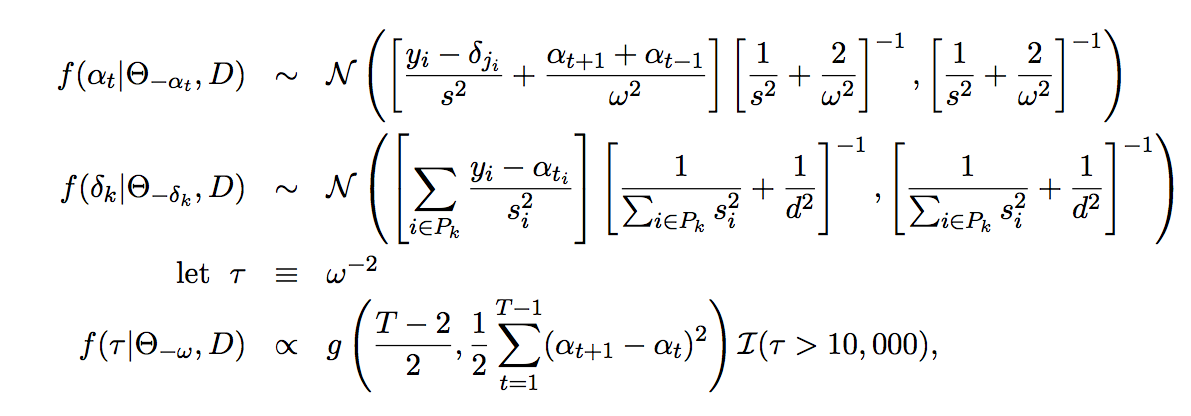
\includegraphics[width=\textwidth]{strauss-gibbs.png}
\end{center}
\end{frame}

\begin{frame}{Example}
\begin{itemize}
	\item Find distributions for popular opinion at each time step in a campaign
	\item Calculate house biases during a campaign
	\item Calculate how much opinion changes over time
\end{itemize}
\end{frame}

\begin{frame}{Further}
\begin{itemize}
\item Why do people vote the way they do? (home-state advantage, correlation within economic zones, etc.)
\item More work on how useful each individual poll has (Nate Silver does a lot of this)
\end{itemize}
\end{frame}

\begin{frame}{Congratulations, you've forecasted a presidential election}
Questions/Comments?
\end{frame}

\end{document}
